\chapter{Implementación de la Solución} \label{Implementacion de Solucion}

En esta sección se detallan las implementaciones tecnológicas de los objetivos del proyecto, a partir de las soluciones mencionadas en el capítulo anterior.
Estos objetivos son la definición de un lenguaje de modelado, que permitirá representar en forma de diagrama el estado de una topología de red. Esto incluye la creación del metamodelo en base a la Definición de Dominio Específico, y la implementación del perfil UML para agregar la extensiones de UML necesarias. 
Además, la implementación de una transformación de modelo a texto, que permita la creación de scripts de configuración a partir de dichos modelos.
Finalmente, la integración de los scripts de configuración generados, con las herramientas de configuración (CMTs), detallando como estas herramientas utilizan los scripts para llevar a cabo la configuración. 

\section{Implementación del modelo UML}
Partiendo de las decisiones que se tomaron en el capitulo anterior, en esta sección se especifica el modelo UML definido para representar el problema objetivo. De forma análoga a la sección Definición de Dominio Específico (Sección \ref{Definicion de Dominio Específico}), se tendrá el metamodelo separado en dos grandes partes, por un lado se encuentra la topología, con nodos lógicos y físicos, y por otro lado se tiene la configuración de estos nodos.

A continuación se describe cada sección por separado, ilustrando las decisiones tomadas en cada una de ellas, para luego mostrar el resultado final del metamodelo, que será el punto de partida para la implementación del perfil UML,y por ende la transformación de modelo a texto.

\subsection{Modelado de la Topología}
El primer componente que se debe considerar dentro de la topología es el de \textbf{Nodo}, dicho componente encapsula todo tipo de nodo, ya sea físico o lógico, por lo que puede representar desde un servidor hasta una instancia de base de datos. 
Este concepto es esencial ya que la configuración que se definirá debe ser capaz de ser aplicada tanto a dispositivos lógicos como físicos, y es necesario que haya un componente en común para representar ambos tipos de nodos independientemente.

De esto, y tal como se explicó anteriormente en la sección Definición de Dominio Específico, surge que se tendrán dos tipos de nodos: físicos y lógicos, lo que se representará con una relación de herencia sobre Nodo, quedando representado en la Figura \ref{fig:uml:node}.

\begin{figure}[htbp]
    \centering
    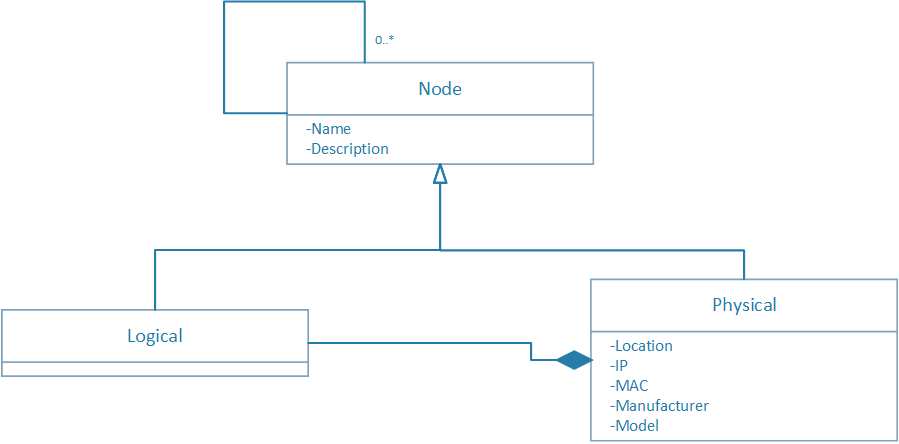
\includegraphics[width=\textwidth]{figures/uml_diagrams/topology_node.png}
    \caption{Representación UML de Nodo.}
    \label{fig:uml:node}
\end{figure}

Además de la relación de herencia de Lógico y Físico sobre Nodo, se tiene una relación de Composición de un nodo Lógico a un nodo Físico, dado que un nodo Físico estará compuesto por varios nodos Lógicos.

También se agregan los atributos considerados principales para el nodo Físico, en el caso del nodo Lógico no se tienen atributos debido a que no existe alguno que se considere esencial y sea común a las especializaciones que se verán luego. 

Por último, el componente de nodo tiene una relación con multiplicidad de cero a varios consigo mismo, con el fin de considerar la relación que existe entre dispositivos de red con servidores, o incluso otros dispositivos de red.

Una vez definido el componente de Nodo, se pasa a definir las especializaciones Físico y Lógico.

\subsubsection{Nodo Físico}
Respecto a los nodos físicos, se mantiene la definición de dominio, es decir, se tienen las especializaciones Servidor (Server), PC, Dispositivo (Device), y se agrega una nueva relación de herencia para los Dispositivos de Red (Network), donde cada uno es una generalización de Router o Switch, y al mismo tiempo, estos son especializaciones de Dispositivo de Red. El metamodelo del componente Físico queda representado en la Figura \ref{fig:uml:physical}.

\begin{figure}[htbp]
    \centering
    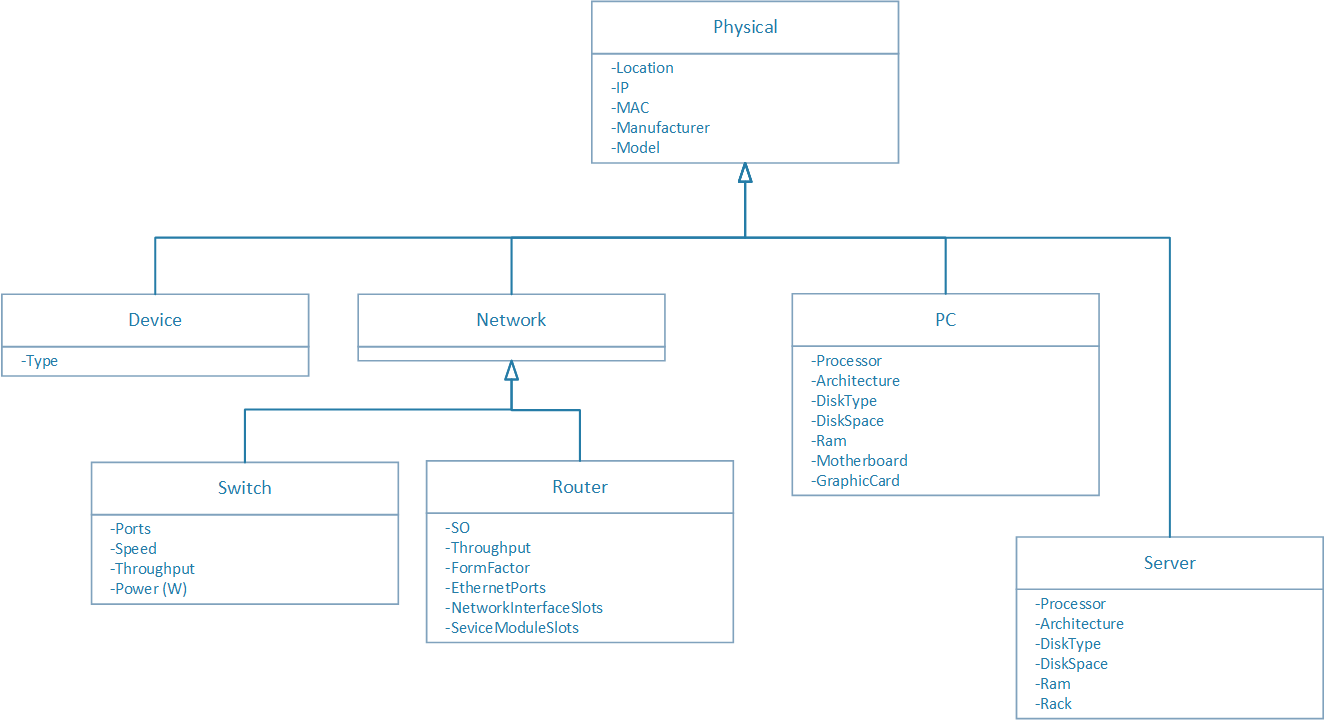
\includegraphics[width=\textwidth]{figures/uml_diagrams/topology_physical.png}
    \caption{Representación UML de Nodo Físico.}
    \label{fig:uml:physical}
\end{figure}

Los atributos de cada componente fueron seleccionados en base a la información de interés para cada uno en el contexto de la topología y configuración, siempre teniendo en cuenta que los principales son heredados del nodo Físico (Physical).

\subsubsection{Nodo Lógico}
De la misma forma, los nodos lógicos fueron seleccionados en base a las decisiones de definición de dominio previamente realizadas, por lo tanto, se considerarán como especialización de Lógico (Lógical): Firewall, Sistema Operativo (OS), Firmware, Ambiente de Ejecución (Runtime), Servidor de Aplicaciones (ApplicationServer), Base de Datos (DBEngine), y Servidor HTTP (HTTPServer).

A su vez, cada clase tiene una especialización en base los componentes de software que se consideraron para cada uno, por lo que se tienen las especializaciones Java para Runtime; Tomcat para ApplicationServer; Postgresql y MySQL para DBEngine; y Apache para HTTPServer. 

En base a esto, el metamodelo del componente Lógico se puede ver en la Figura \ref{fig:uml:logical}.

\begin{figure}[htbp]
    \centering
    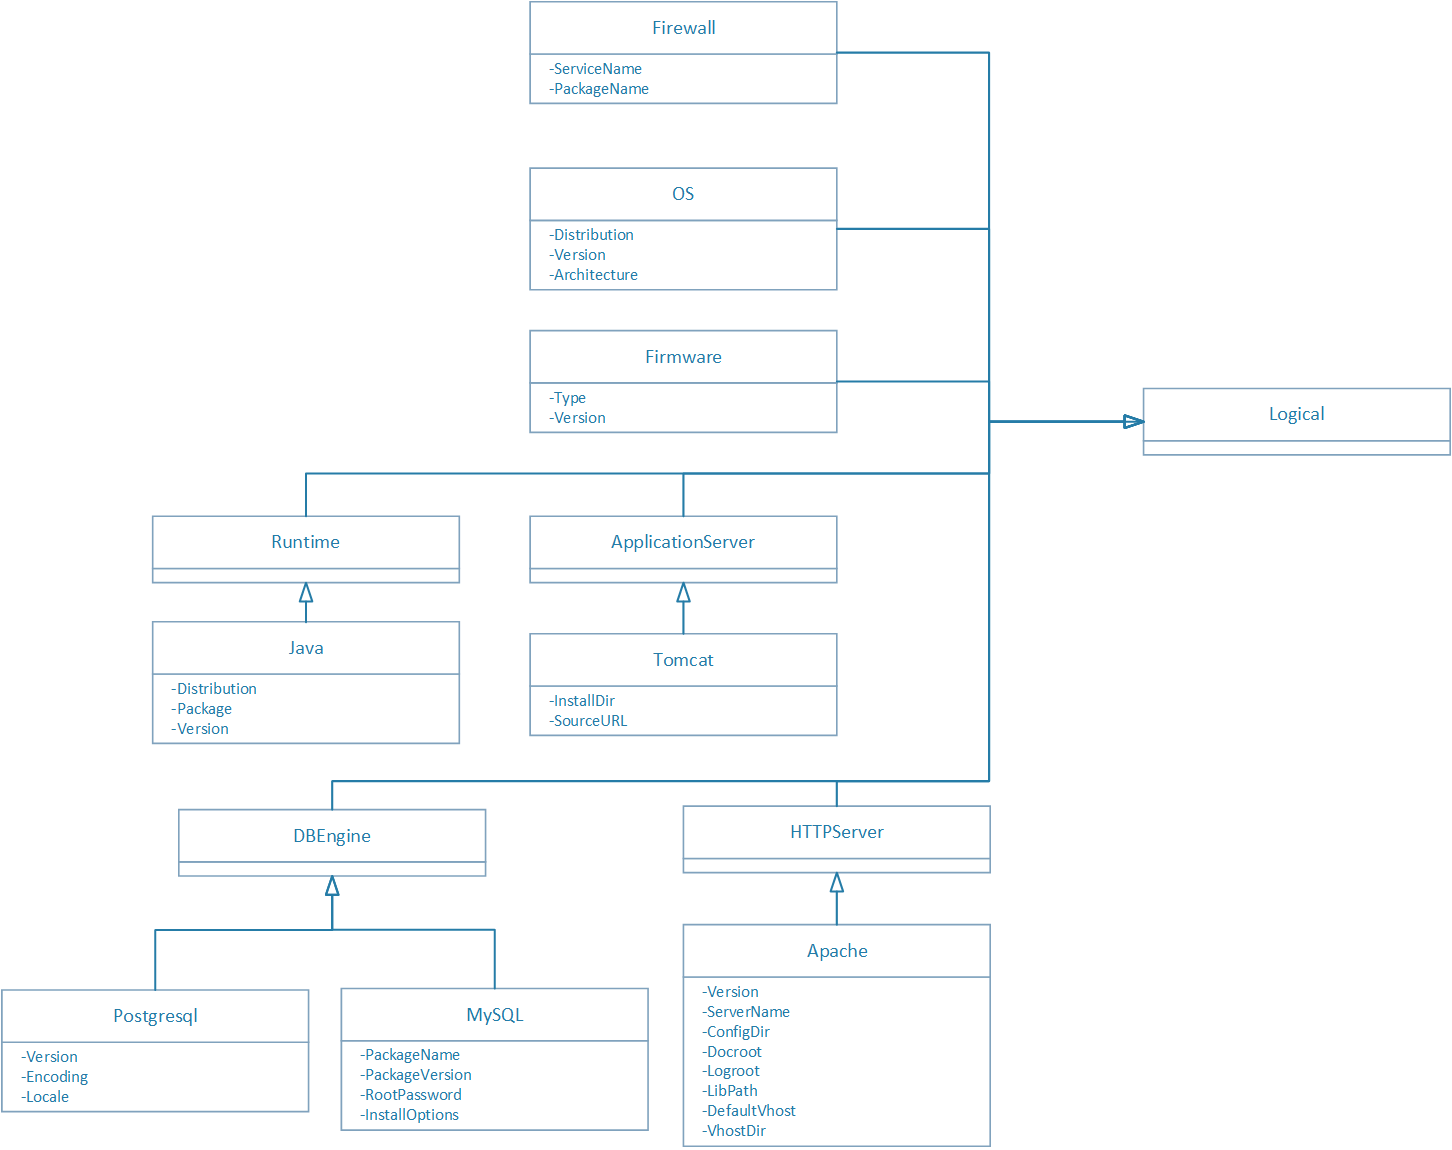
\includegraphics[width=\textwidth]{figures/uml_diagrams/topology_logical.png}
    \caption{Representación UML de Nodo Lógico.}
    \label{fig:uml:logical}
\end{figure}

Los atributos de Sistema Operativo y Firmware fueron seleccionados en base a la información básica y necesaria en el contexto del problema, ya que serán utilizados de forma puramente informativa. 
Sin embargo, los atributos de los componentes de software debieron ser seleccionados cuidadosamente, tomando como referencia el soporte brindado por los CMTs a utilizar. Dichos componentes fueron seleccionados a partir del soporte brindado por los manejadores de configuración, por lo tanto, sus atributos se deben corresponder con los atributos que estos dispongan. 
En base al estudio de los diferentes componentes en cada CMT (Puppet, Chef) se obtuvieron los atributos que se muestran en la imagen.

\subsubsection{Topología}
Una vez definidos los metamodelos de Nodo, Físico y Lógico, sólo resta unificar los resultados para obtener el metamodelo de la topología, en la Figura \ref{fig:uml:topology}.

\begin{figure}[htbp]
    \centering
    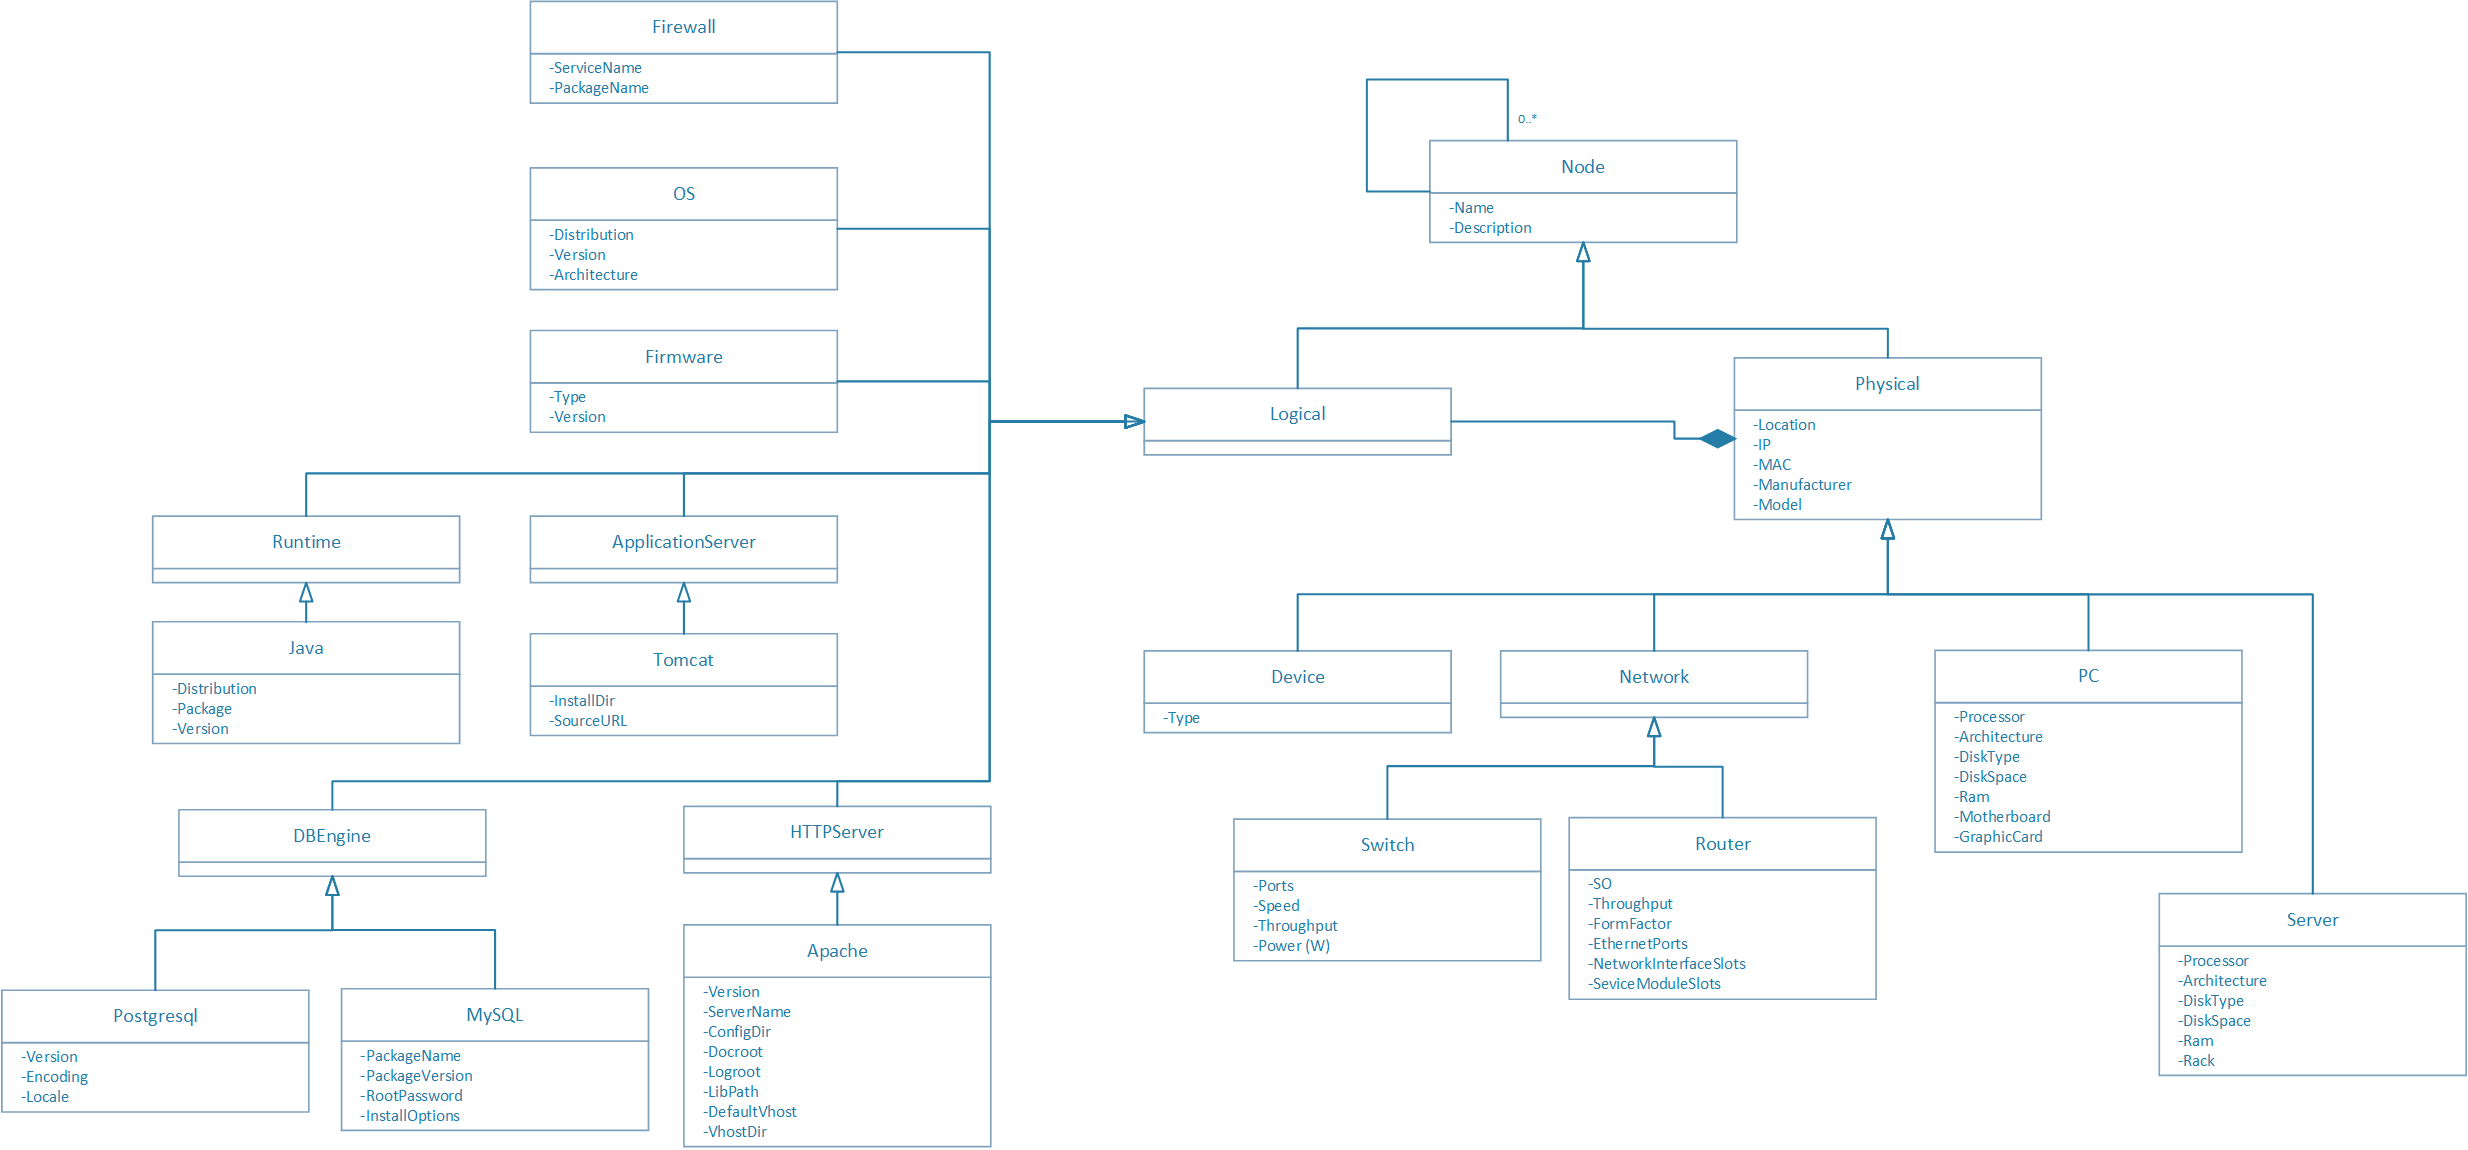
\includegraphics[width=\textwidth]{figures/uml_diagrams/topology.png}
    \caption{Representación UML de la Topología.}
    \label{fig:uml:topology}
\end{figure}


\subsection{Modelado de la Configuración}
En el caso de la configuración, como se discutió previamente, se tendrán distintos tipos. El tipo de configuración más básico es el de configuración Abierta (Open), que consiste simplemente de una descripción, ya sea a alto nivel o con opciones de configuración específicas de cualquier Nodo, se utiliza particularmente para Nodos que no poseen una configuración aplicable y se desea tener un registro, por ejemplo para los componentes Dispositivo.

Luego, se tiene la configuración de Registro (Registry), que aplica solamente a los nodos con Sistema Operativo Windows, y son configuraciones que se pueden aplicar a las entradas de dichos registros.

También se tiene configuración de tipo Archivo (File), que representa las diferentes acciones que se pueden realizar sobre los archivos del sistema.

Finalmente, se tiene una especialización para cada tipo de componente de software, los cuales se corresponderán con los componentes de Nodo Lógico que se mencionaron previamente. 
Cada instancia de configuración de estas herramientas representa una instancia del componente de software asociado a un componente del Nodo Lógico. De esta forma, por ejemplo, se puede tener una instancia de nodo Lógico de base de datos (DBEngine), el cual a su vez puede tener varias instancias de una base de datos, dicho de otra forma, un servicio de base de datos (MySQL) podrá tener varias instancias de base de datos (development, production).
Lo mismo aplica para cada uno de los componentes de software, cada instancia de Nodo Lógico potencialmente puede tener asociadas varias instancias de Configuración.

Con el mismo análisis que se realizó para definir los atributos de los componentes Lógicos, se seleccionaron los atributos disponibles en los componentes de configuración. Los atributos de cada componente representan las capacidades de configuración que brinda la herramienta de manejo de configuración (CMTs) para dicho componente.

Con base en lo anterior, el metamodelo final del componente de Configuración tendrá la forma de la Figura \ref{fig:uml:configuration}.

\begin{figure}[htbp]
    \centering
    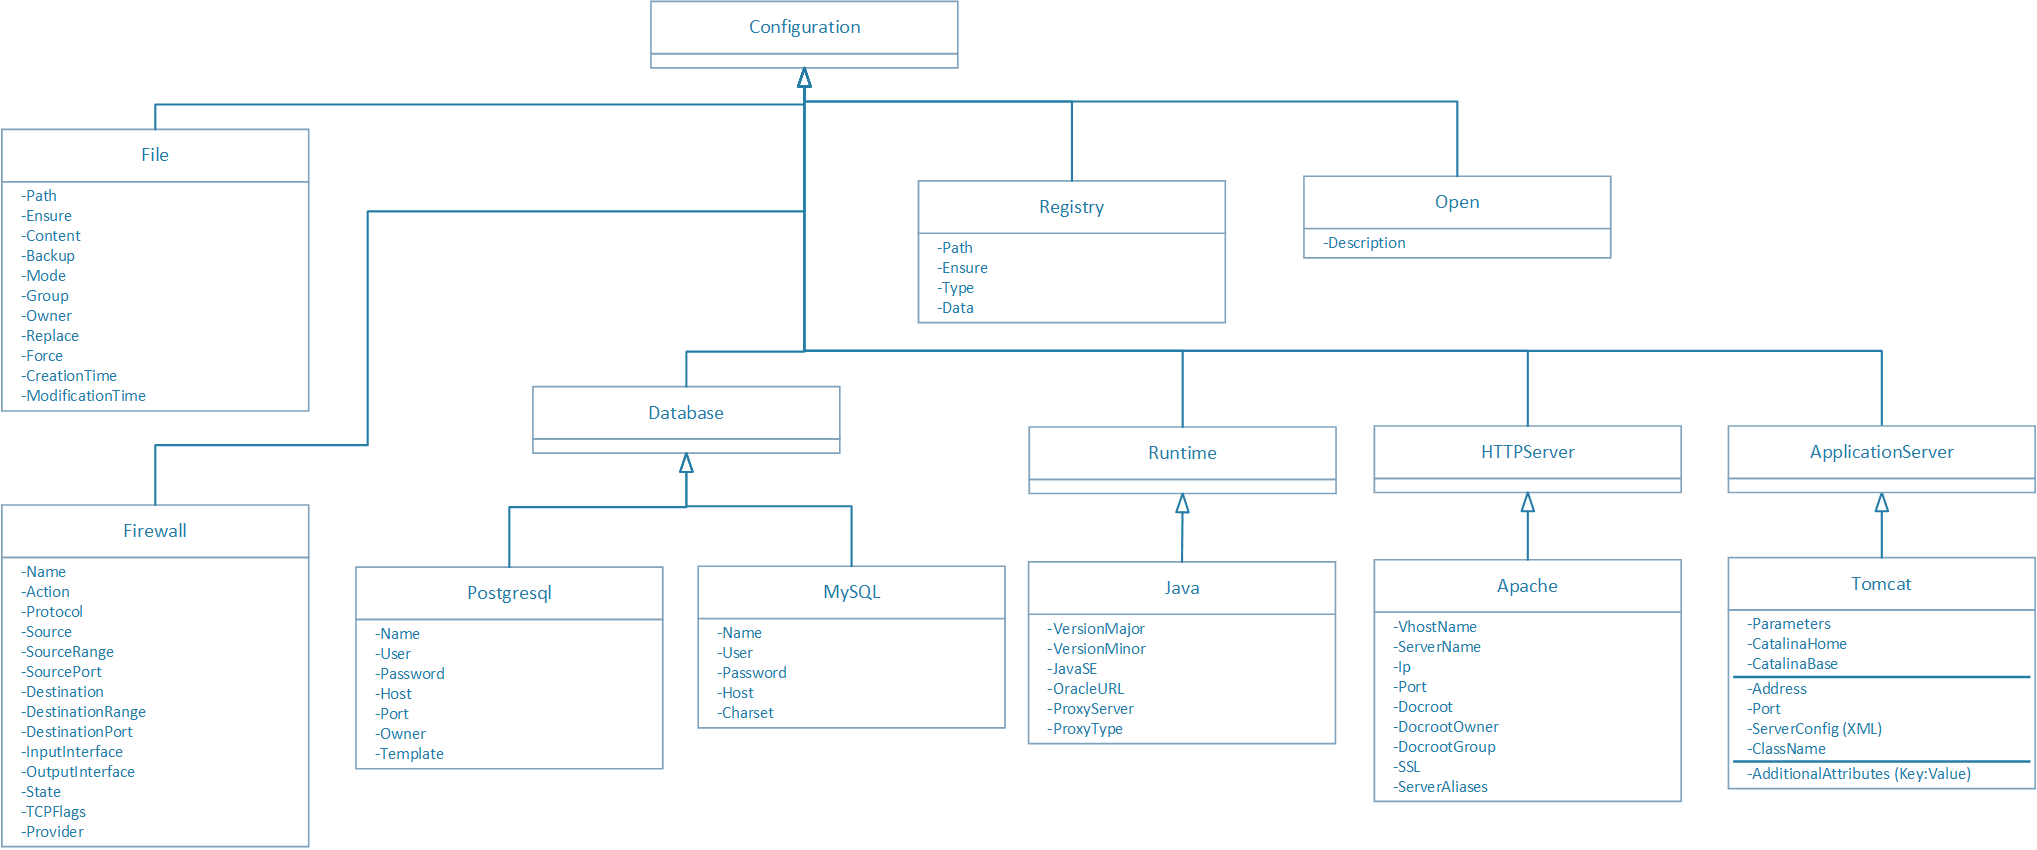
\includegraphics[width=\textwidth]{figures/uml_diagrams/configuration.png}
    \caption{Representación UML de Configuración.}
    \label{fig:uml:configuration}
\end{figure}

\subsection{Modelado de la Solución}
Una vez definidos los componentes de Topología y Configuración, que forman la solución objetivo, sólo resta unificar estos resultados en base a la relación de los mismos. En este caso, se tiene que los Nodos podrán tener varias instancias del componente de Configuración, por lo que dicha relación tendrá multiplicidad de cero a varios. 

Por otro lado, también se debe considerar la posibilidad de tener un grupo de Nodos Físicos con su respectiva Configuración, esto es especialmente útil en los casos que se tienen conjuntos de dispositivos, y se desea que compartan una misma configuración. Para evitar que cada dispositivo necesite ser configurado individualmente, se agrega la multiplicidad de uno a varios con el componente de Configuración, de forma de que cada grupo de nodos pueda tener asociado una cantidad de instancias de Configuración, cumpliendo el propósito deseado.

El metamodelo que representará la solución propuesta se puede ver en la Figura \ref{fig:uml:solution}. Se obviaron los componentes de bajo nivel mostrados previamente con el fin de representar de forma más clara la solución.

\begin{figure}[htbp]
    \centering
    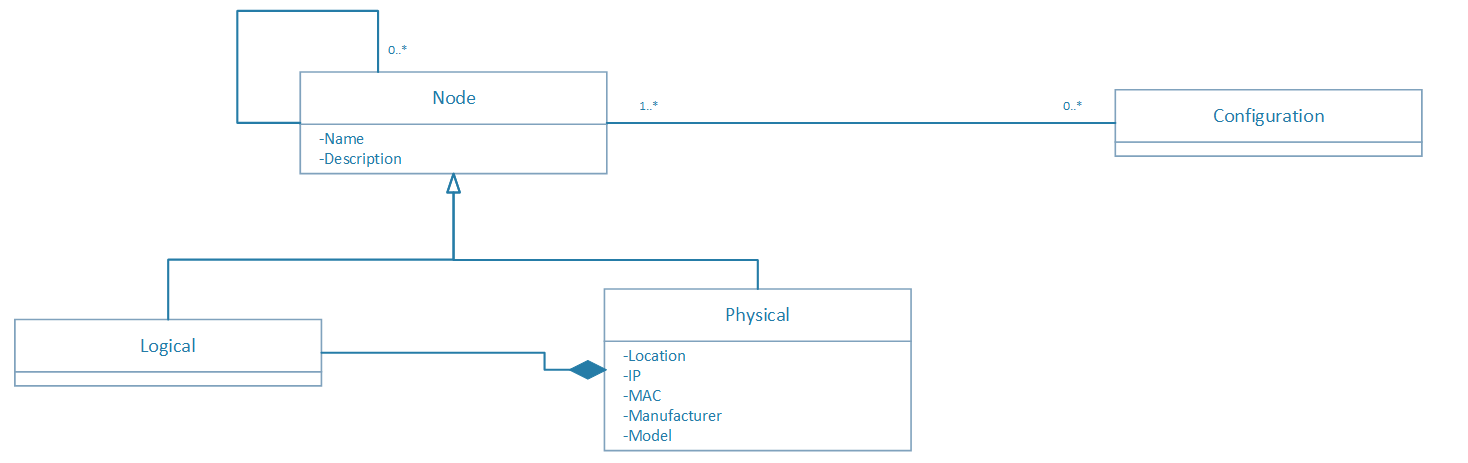
\includegraphics[width=0.8\textwidth] {figures/uml_diagrams/solution.png}
    \caption{Representación UML de la solución propuesta.}
    \label{fig:uml:solution}
\end{figure}

\section{Implementación del Perfil UML}
Partiendo de la base del diagrama de la solución en la sección anterior, se puede pasar a la implementación del perfil UML. Para realizar dicha implementación se utilizará el entorno de modelado Papyrus, extensión de Eclipse.

Tal como se discutió en secciones previas, se utilizará el perfil para extender los componentes UML análogos a los presentados en la solución, por un lado se extenderá el componente \textbf{Device}, para poder representar los \textbf{Nodos Físicos}, y el componente \textbf{ExecutionEnvironment} para representar los \textbf{Nodos Lógicos}, y por otro lado se extenderá el componente \textbf{Artifact} representando los componentes de \textbf{Configuración}.

Las extensiones de los elementos UML se realizan utilizando estereotipos, que permiten agregar o crear nuevos elementos del modelo a partir de los existentes. Se necesitará crear un estereotipo para cada metaclase a extender, en este caso dichas metaclases son \textbf{Device}, \textbf{ExecutionEnvironment}, y \textbf{Artifact}, y los estereotipos a crear, para extender cada metaclase, serán \textbf{Physical}, \textbf{Logical}, y \textbf{Configuration}, respectivamente. Cabe notar que se obvio la implementación del estereotipo \textbf{Node}, que sí estaba presente en el diagrama de la solución analizada en la sección anterior. Esto se debe a que se consideró que dicha extensión no aportaba valor, dado que el elemento UML que se necesita extender, también llamado \textbf{Node}, posee la información necesaria, es decir, el nombre.

Para realizar la implementación de los estereotipos, basta con importar la metaclase a extender, y utilizar el componente de \textbf{Stereotype} que provee Papryrus para indicar el nombre y atributos de la extensión.
Esto se realiza creando un proyecto Papyrus de tipo \textbf{Perfil UML}, que provee todas las herramientas necesarias para la implementación.

La extensión de los elementos mencionados previamente, utilizando estereotipos, se encuentra en la Figura \ref{fig:profile:base_stereotypes}.

\begin{figure}[htbp]
    \centering
    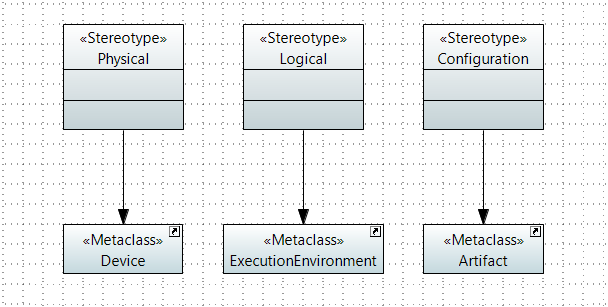
\includegraphics[width=\textwidth]{figures/profile_implementation/stereotypes_0.png}
    \caption{Estereotipos aplicados a Device, ExecutionEnvironment, y Artifact.}
    \label{fig:profile:base_stereotypes}
\end{figure}

Partiendo de esta base se continúa agregando el resto de los elementos de la solución, y dado que la implementación de cada estereotipo es independiente, se separa cada uno de ellos en una sección a continuación.

\subsection{Nodos Físicos}
En la implementación del estereotipo \textbf{Physical}, aplicado a la metaclase \textbf{Device}, se utilizan los elementos definidos previamente en el diagrama UML, estos son Servidor (\textbf{Server}), \textbf{PC}, Dispositivo \textbf{(Peripheral)}, y los Dispositivos de Red \textbf{(NetworkDevice)}, \textbf{Router} y \textbf{Switch}. Los elementos Peripheral, Server, Network Device, y PC son especializaciones del nodo Físico (\textbf{Physical)}, y a su vez, Switch y Router son especializaciones de Network Device. Los atributos se agregan de acuerdo a como fueron seleccionados en el análisis de la solución, y se les asigna el tipo adecuado.

El diagrama de estereotipos definidos resultante se puede ver en la Figura \ref{fig:profile:device}.

\begin{figure}[htbp]
    \centering
    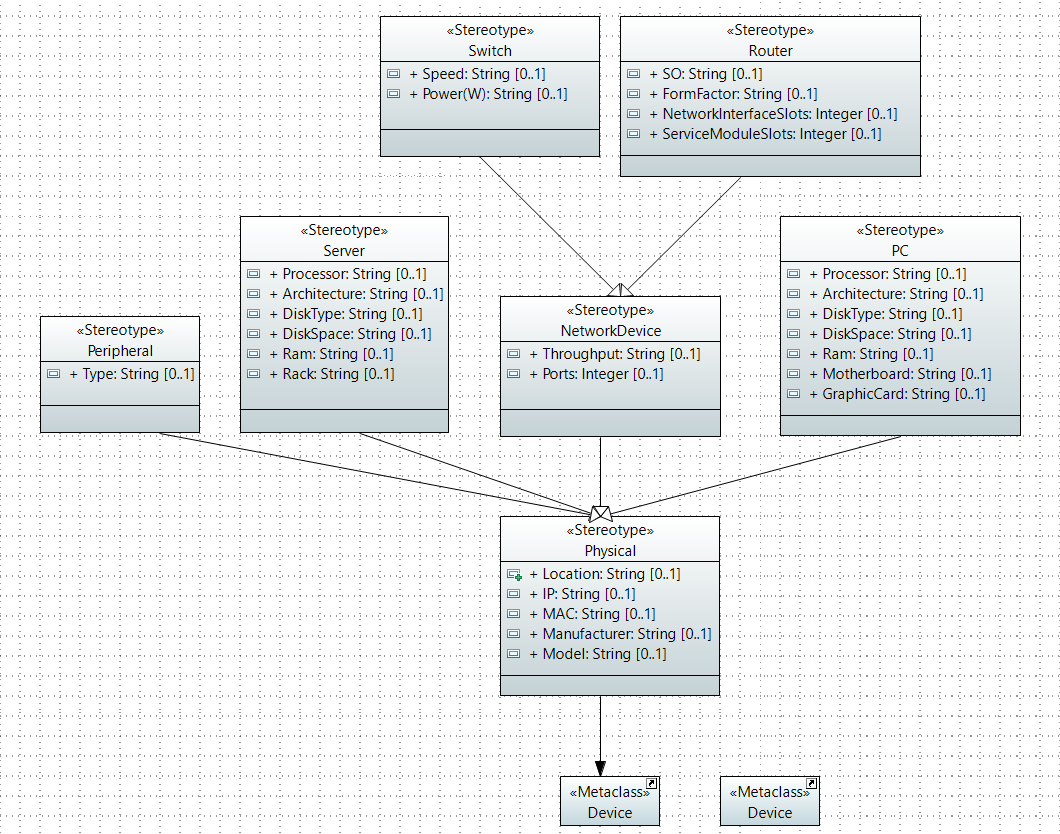
\includegraphics[width=\textwidth]{figures/profile_implementation/stereotypes_device.png}
    \caption{Diagrama de Estereotipos Physical.}
    \label{fig:profile:device}
\end{figure}

\subsection{Nodos Lógicos}
En el caso de los nodos Lógicos, el estereotipo \textbf{Logical} es aplicado a la metaclase \textbf{ExecutionEnvironment}, esto permite que los nodos Lógicos puedan ser asignados a los nodos Físicos, al ser heredado de la relación entre Device y ExecutionEnvironment. De la misma forma que con los nodos Físicos, se utiliza como base el diagrama UML definido. Las especializaciones se realizan de la misma forma, en base a los elementos definidos con anterioridad. También se utilizan los atributos definidos, agregando para cada uno el tipo correspondiente, tal como se aprecia en la Figura \ref{fig:profile:logical}.

\begin{figure}[htbp]
    \centering
    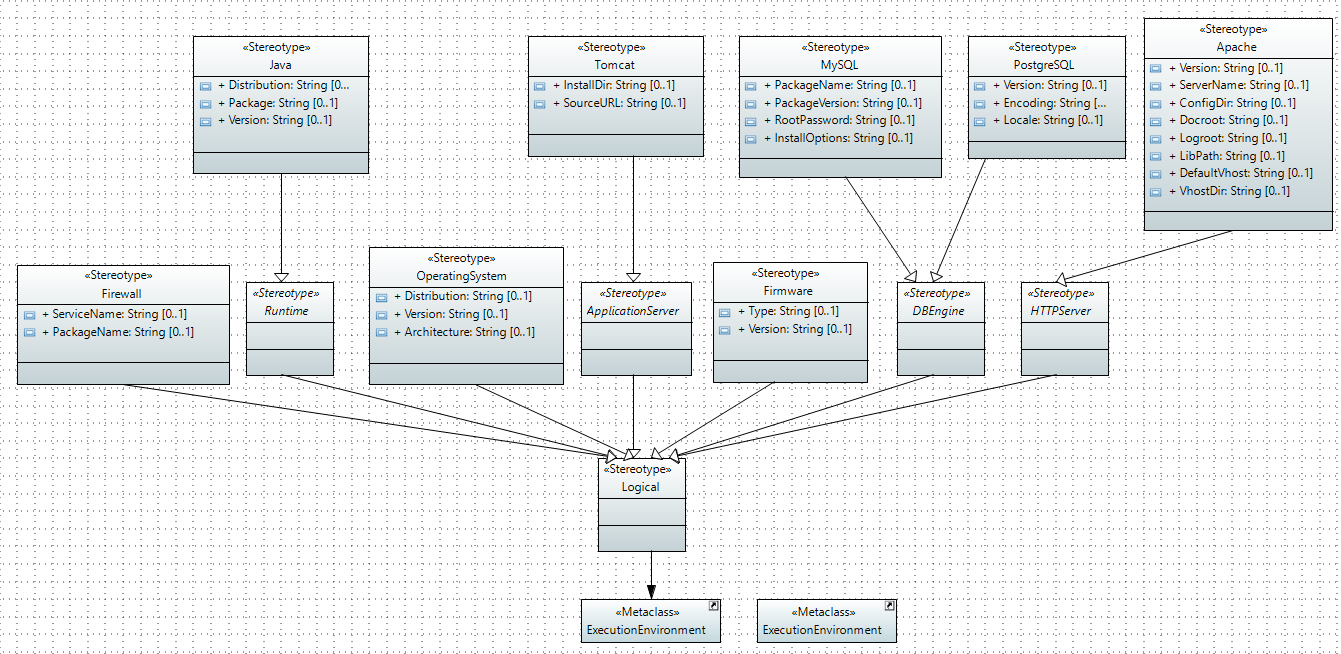
\includegraphics[width=\textwidth]{figures/profile_implementation/stereotypes_execEnv.png}
    \caption{Diagrama de Estereotipos Logical.}
    \label{fig:profile:logical}
\end{figure}

\subsection{Configuración}
Finalmente se tiene la definición de Configuración, en este caso el estereotipo \textbf{Configuration} es aplicado a la metaclase \textbf{Artifact}. De esta forma, una Configuración puede ser desplegada (\textit{deployed}) en un nodo Lógico, ya que la relación de \textbf{deployment} es heredada por ser extensiones de las metaclases Artifact, y ExecutionEnvironment respectivamente.

La implementación del estereotipo se realiza a partir del análisis anterior, aunque en este caso es necesario realizar cambios con respecto al diagrama original. En dicho diagrama se puede ver que varios elementos bajo el nodo Logical comparten el mismo nombre con otros elementos bajo el metamodelo Configuration, por ejemplo, existen dos metamodelos con nombre Java.
Con el fin de diferenciar dichos nombres en la definición de estereotipos, en este caso se cambian estos nombres:
\begin{itemize}
    \item Apache se renombra a ApacheVhost
    \item Firewall se renombra a FirewallRule
    \item Java se renombra a JavaOracle
    \item Tomcat se renombra a TomcatApp
    \item Postgresql se renombra a PSQLDB
    \item MySQL se renombra a MySQLDB
\end{itemize}

Esto expresa de mejor manera lo que representa cada elemento, y a su vez elimina cualquier lugar a confusión entre dichos elementos. Por esta razón también se modifico el nombre de configuración Libre, de \textbf{Open} a \textbf{FreeForm}, el cual resulta más expresivo.

Con este problema resuelto, se continúa con la implementación agregando los atributos correspondientes a cada estereotipo, con su tipo correspondiente.
El resultado final del diagrama de estereotipos se encuentra en la Figura \ref{fig:profile:artifact}.

\begin{figure}[htbp]
    \centering
    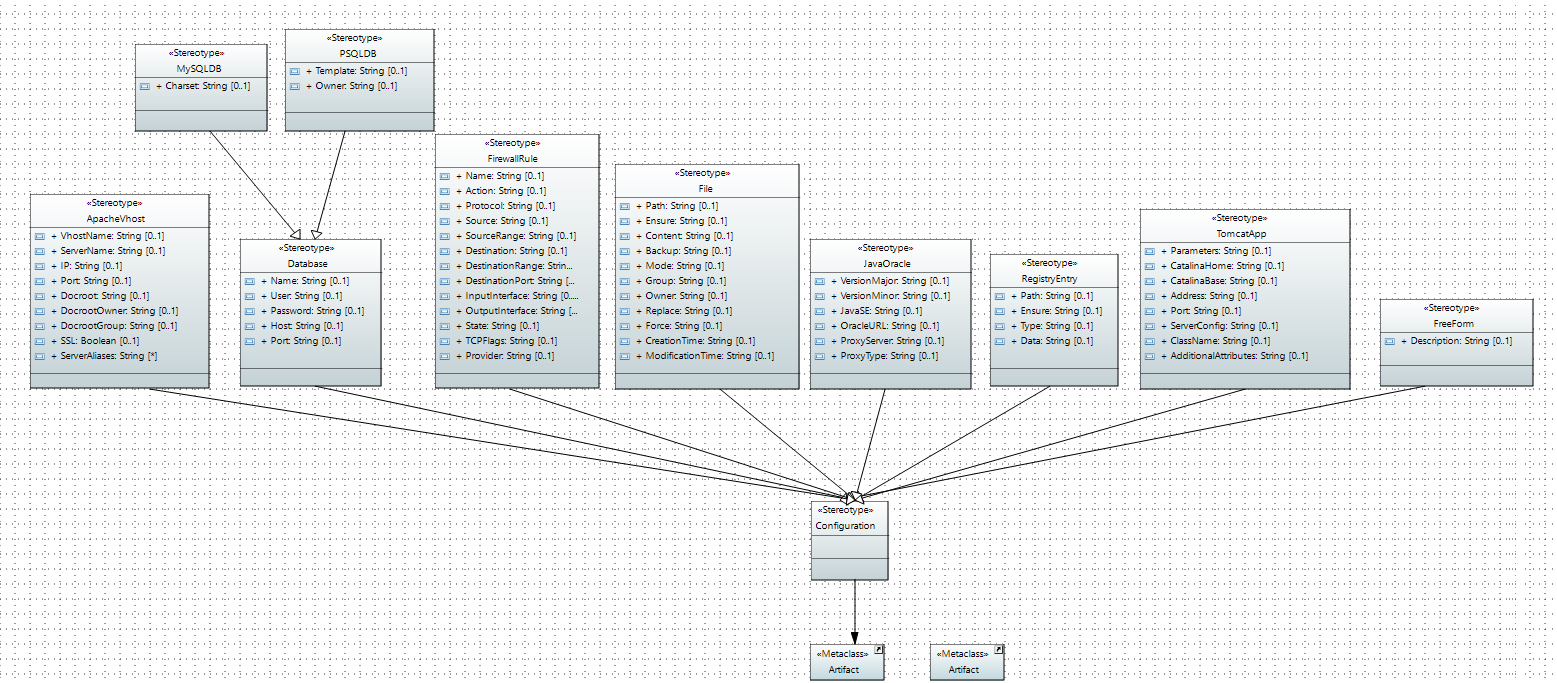
\includegraphics[width=\textwidth]{figures/profile_implementation/stereotypes_artifact.png}
    \caption{Diagrama de Estereotipos Configuration.}
    \label{fig:profile:artifact}
\end{figure}

\subsection{Restricciones}
Como detalle final a la implementación del perfil, es necesario agregar las restricciones (\textbf{Constrains}) adecuadas. En este caso, las restricciones que se deben agregar son aquellas que relacionan a la Configuración con los nodos Lógicos. Los elementos de Configuración que se corresponden a un componente de nodo Lógico, es decir, ApacheVhost, FirewallRule, JavaOracle, TomcatApp, PSQLDB, y MySQLDB, deben ser desplegados sobre su correspondiente elemento de software, de forma de evitar que elementos incompatibles sean relacionados entre sí.
Para ello se crea una restricción (Constrain) para cada uno de estos estereotipos, que explicita el tipo de estereotipo al cuál puede ser desplegado.

A continuación se presenta una descripción de las restricciones agregadas a cada componente de Configuración, asociado a su correspondiente componente Lógico:

\begin{itemize}
    \item ApacheVhost: sólo puede ser desplegado a un componente lógico Apache
    \item MySQLDB: sólo puede ser desplegado a un componente lógico MySQL
    \item PSQLDB: sólo puede ser desplegado a un componente lógico PostgreSQL
    \item FirewallRule: sólo puede ser desplegado a un componente lógico Firewall
    \item JavaOracle: sólo puede ser desplegado a un componente lógico Runtime
    \item TomcatApp: sólo puede ser desplegado a un componente lógico Tomcat
\end{itemize}

El resultado final del diagrama de estereotipos \textbf{Configuration}, incluyendo las restricciones, esta representado en la Figura \ref{fig:profile:artifact_final}.

\begin{figure}[htbp]
    \centering
    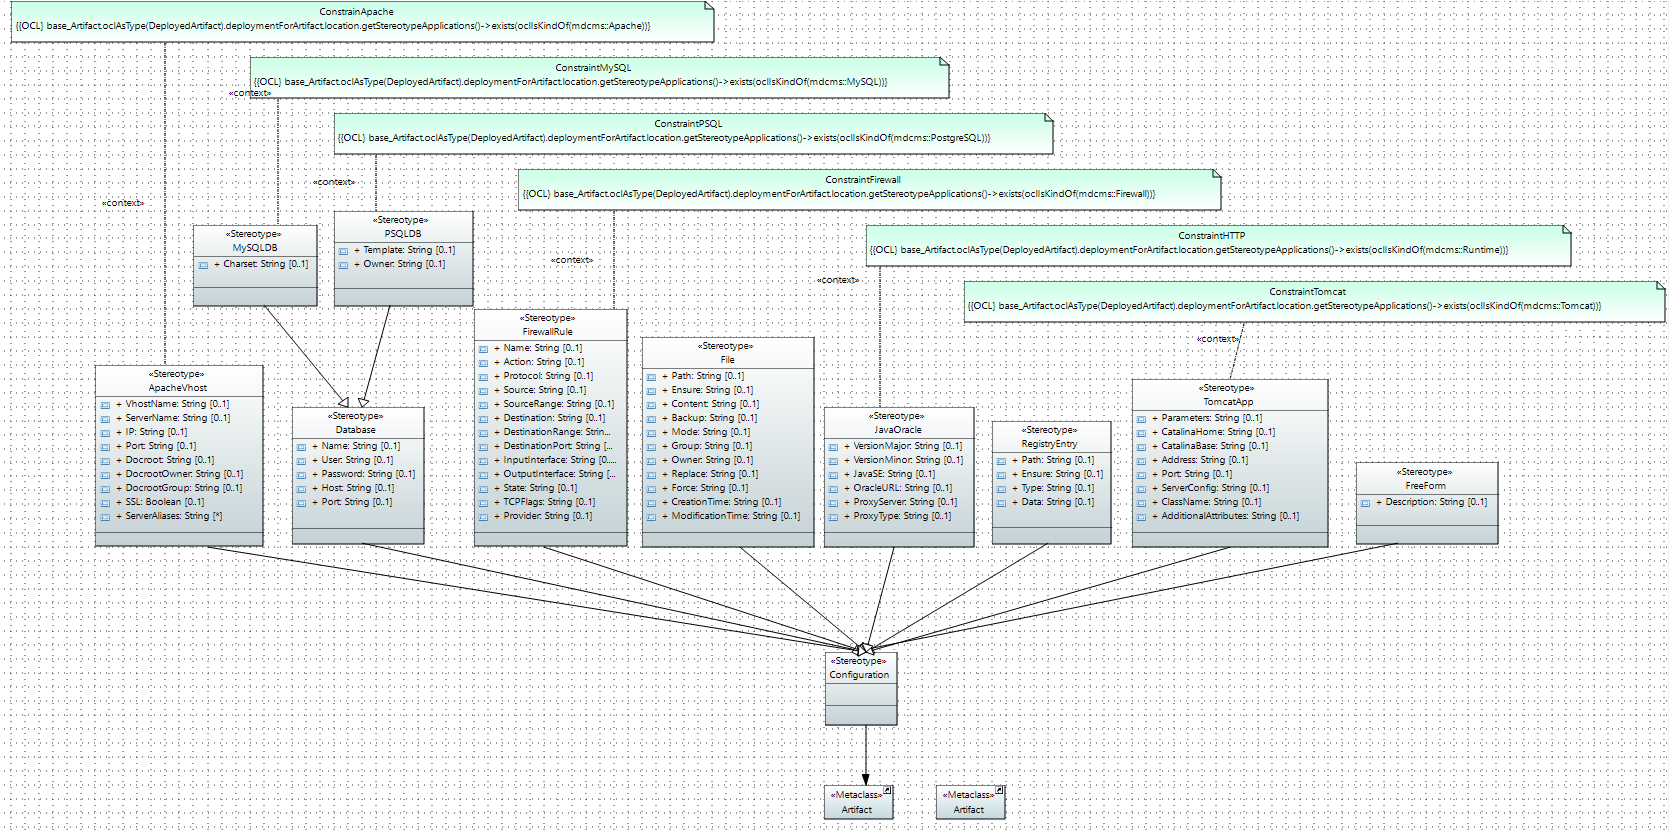
\includegraphics[width=\textwidth]{figures/profile_implementation/stereotypes_artifact_2.png}
    \caption{Diagrama de Estereotipos Configuration con restricciones.}
    \label{fig:profile:artifact_final}
\end{figure}

\subsection{Implementación del Perfil como plugin}

Una vez realizado el perfil, es necesario instalarlo como plug-in, para ello se utiliza un generador de modelos EMF (Eclipse Modeling Framework). Primero se crea un proyecto EMF, utilizando como base el proyecto Papyrus y el perfil UML existente. Esto generará los archivos descriptores Ecore y Genmodel basados en UML, que son las dos partes que componen un meta-modelo EMF. Luego, en base al Genmodel generado, se podrá generar el código del modelo para el perfil UML.

Finalmente, se agregan las extensiones necesarias para el plug-in, estas incluyen el paquete Ecore generado, que se agrega automáticamente en el proceso de generación del modelo con EMF; un mapeo de URI para el modelo Ecore que indica el proyecto origen y el plug-in destino del proyecto; y los puntos de extensión (extension points) para el perfil UML, que poseen el nombre que tendrá el perfil, así como la ubicación del perfil implementado (archivo .profile.uml). Esto se puede ver en la Figura \ref{fig:profile:extensions}.

\begin{figure}[H]
    \centering
    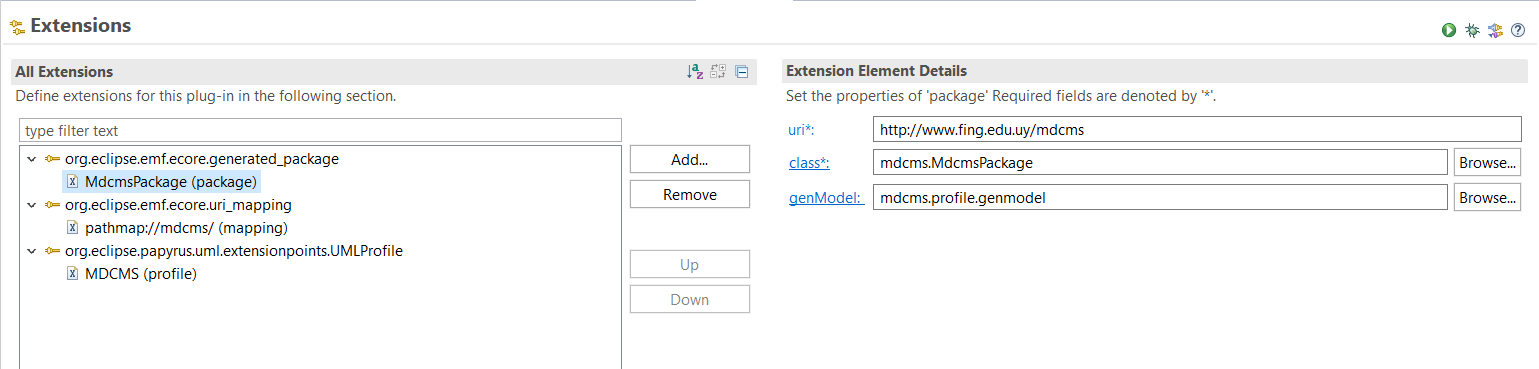
\includegraphics[width=\textwidth]{figures/profile_implementation/profile_extensions.png}
    \caption{Extensiones necesarias para el perfil como plug-in.}
    \label{fig:profile:extensions}
\end{figure}

Una vez definidos los pasos anteriores, simplemente se exporta el proyecto como plug-in, con la funcionalidad de Exportar que provee Eclipse para Desarrollo de Plug-ins, indicando la modalidad de exportación (directorio, archivo, o instalación local). (Figura \ref{fig:profile:plugin_export})

\begin{figure}[H]
    \centering
    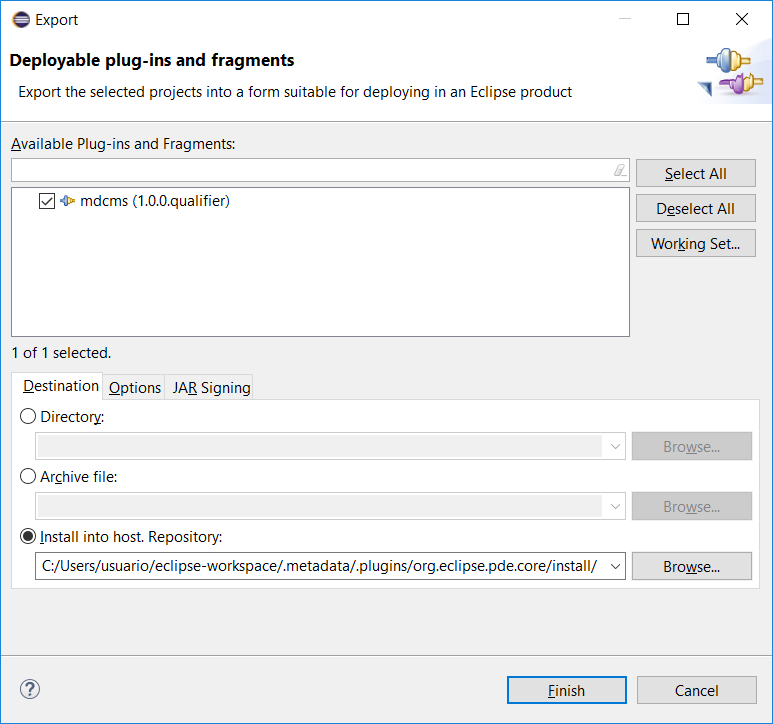
\includegraphics[width=0.8\textwidth]{figures/profile_implementation/profile_export.png}
    \caption{Exportación del proyecto como plug-in.}
    \label{fig:profile:plugin_export}
\end{figure}

Luego de la instalación, al crear un nuevo modelo se tendrá la opción de aplicar el perfil UML creado, como se puede ver en la Figura \ref{fig:profile:apply}.

\begin{figure}[htbp]
    \centering
    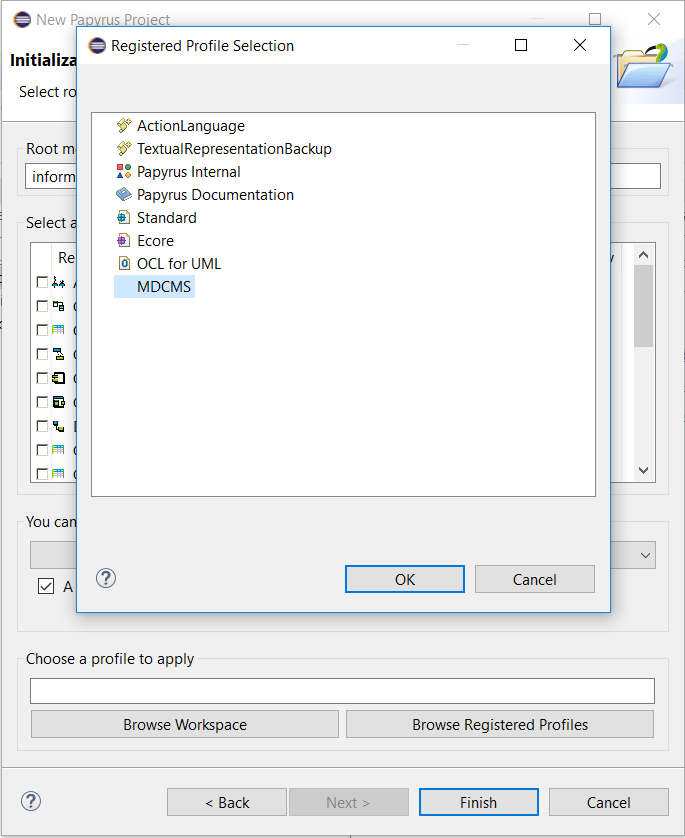
\includegraphics[width=0.8\textwidth]{figures/profile_implementation/profile_installed.png}
    \caption{Aplicación del plug-in exportado.}
    \label{fig:profile:apply}
\end{figure}

\section{Implementación de la Transformación}

La transformación de modelo a texto se realizará utilizando la herramienta Acceleo, extensión de Eclipse, que permite generación de código en base a plantillas. Para los objetivos de este proyecto, la salida generada por la transformación fue dirigida a Puppet como CMT (Configuration Manager Tool) principal, esto quiere decir que los archivos de configuración generados tienen la sintaxis de dicha herramienta.

De igual forma que en capítulos anteriores, este se podría separar según nodo Físico, Lógico y Configuración, sin embargo, en este caso es conveniente hacer la distinción a partir del tipo de salida que se va a generar. 

Por un lado se tienen los scripts de configuración que serán utilizados por un CMT, es decir, los componentes de software que fueron analizados e incluidos en el diseño de la solución y definidos en el perfil UML; y por otro lado se tienen los textos planos que serán utilizados puramente como información, esto incluye, por ejemplo, los componentes físicos y la configuración de tipo Libre (FreeForm). 
Se realizará una transformación para cada una de estas clases, por un lado se tendrá la transformación \textbf{mdcms2puppet} que generará los archivos de configuración a ser utilizados por Puppet (con extensión \textbf{.pp}), mientras que los archivos informativos (con extensión \textbf{.txt}) serán generados por la transformación \textbf{mdcms2info}.

La salida generada por la transformación \textbf{mdcms2puppet} se organizó en base a lo anterior, y teniendo en cuenta la clase de elemento que genera dicha transformación. En primer lugar se genera un archivo Puppetfile que contiene los módulos que se necesitan instalar para la utilización en Puppet, y también un archivo \textbf{site.pp} (manifests/site.pp), que tendrá la información de los nodos existentes en la topología, esto será utilizado para declarar los diferentes nodos en Puppet, incluyendo la configuración correspondiente a cada uno.

En la Figura \ref{fig:transformation:site} se puede ver el modelo origen, el código de la transformación para esos elementos, y el resultado obtenido de dicha transformación.

\begin{figure}[htbp]
    \centering
    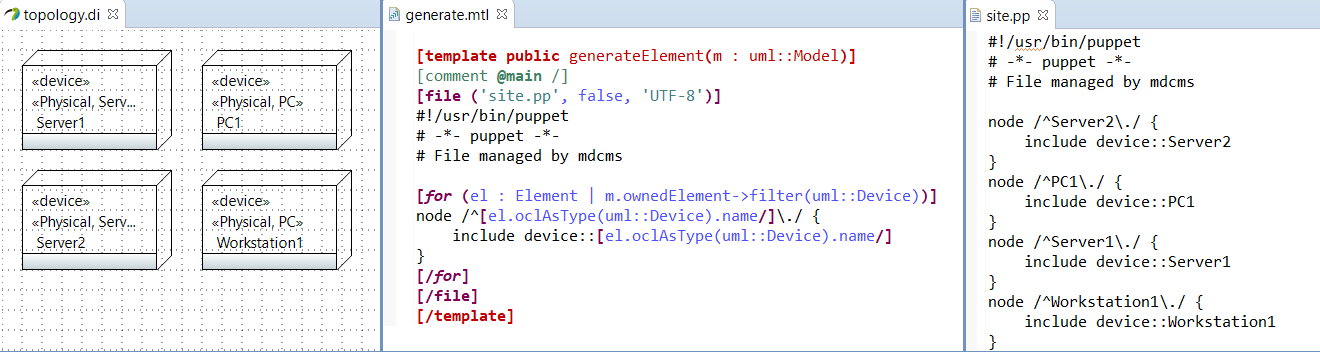
\includegraphics[width=\textwidth]{figures/transformation_implementation/site.png}
    \caption{Ejemplo de un modelo origen, una transformación, y su salida correspondiente.}
    \label{fig:transformation:site}
\end{figure}

Tal como se puede apreciar, se genera un nodo de Puppet por cada componente en el modelo de origen, esto se debe a la funcionalidad en modo de plantilla de Acceleo, que permite obtener la salida de la forma que está plasmada en el archivo de generación.

Este archivo es el punto de partida de la configuración, la información de cada nodo, ya sea físico o lógico, se encontrará bajo \textbf{modules/device/manifests}, mientras que los elementos de configuración serán creados en el directorio \textbf{modules/configurations/manifests}.

Por otro lado, para la transformación \textbf{mdcms2info}, bajo el directorio \textbf{Information} se encontrarán los archivos de texto plano, cuyo fin es puramente informativo, mientras que en el directorio \textbf{Configuration} se encontrarán los archivos generados a partir de los componentes FreeForm. Esta estructura facilita el manejo de dichos archivos, organizándolos en base a su comportamiento. En la Figura \ref{fig:transformation:structure} se encuentra dicha estructura de archivos a alto nivel.

\begin{figure}[htbp]
    \centering
    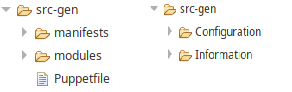
\includegraphics[width=0.5\textwidth]{figures/transformation_implementation/structure.png}
    \caption{Estructura de archivos generada por cada transformación.}
    \label{fig:transformation:structure}
\end{figure}

La transformación y estructura de estos elementos se analiza en las siguientes secciones.

\subsection{Generación de Información}
Los elementos del modelo que pueden generar archivos de información son los siguientes:
\begin{itemize}
    \item Cualquier nodo físico: Server, PC, Router, Switch, y Peripheral
    \item Dentro de los nodos lógicos solamente OperatingSystem y Firmware.
    \item En el caso de la configuración, FreeForm es el único que aplica.
\end{itemize}

Como se mencionó previamente, la generación de estos elementos se ubicará en el directorio \textbf{Information}, con la excepción de FreeForm los cuales se encontrarán bajo \textbf{Configuration}. Para los primeros se creará un directorio por cada nodo Físico, y en dicho directorio se encontrará su información correspondiente, así como la de todos los nodos lógicos que pertenezcan a este nodo. Esto se puede ver en la Figura \ref{fig:transformation:information_example}.

\begin{figure}[htbp]
    \centering
    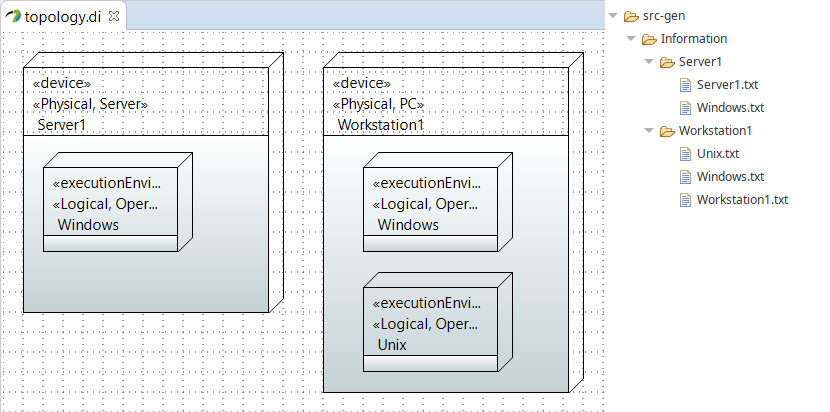
\includegraphics[width=\textwidth]{figures/transformation_implementation/information_example0.png}
    \caption{Ejemplo de generación de archivos de Información.}
    \label{fig:transformation:information_example}
\end{figure}

La generación de estos archivos de configuración se realiza en base a los atributos definidos en el modelo, gracias a la modalidad de transformación de Acceleo, fácilmente se pueden definir los atributos de forma clave-valor en el archivo de texto, en este caso se utiliza una función auxiliar para dar este formato. El código utilizado para esta transformación se puede ver en la Figura \ref{fig:transformation:generator}.

\begin{figure}[htbp]
    \centering
    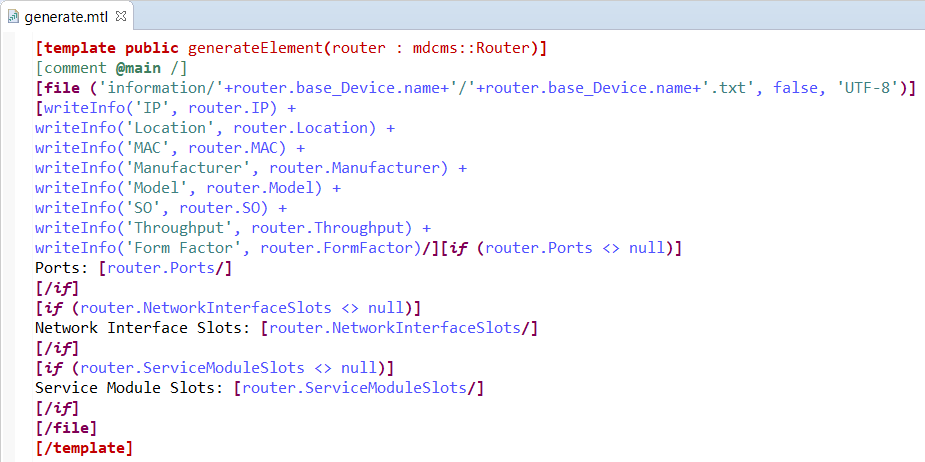
\includegraphics[width=\textwidth]{figures/transformation_implementation/information_generator.png}
    \caption{Código de la generación del archivo de información para el elemento Router.}
    \label{fig:transformation:generator}
\end{figure}

La Figura \ref{fig:transformation:information_generated} muestra el resultado de la transformación del modelo presentado previamente (Figura \ref{fig:transformation:information_example}).

\begin{figure}[htbp]
    \centering
    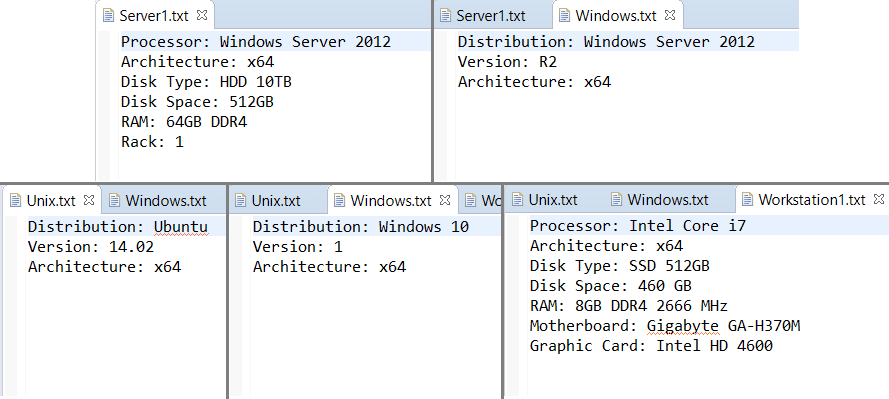
\includegraphics[width=\textwidth]{figures/transformation_implementation/information_example1.png}
    \caption{Resultado de la transformación del modelo en la Figura \ref{fig:transformation:information_example}.}
    \label{fig:transformation:information_generated}
\end{figure}

Esta definición es análoga para todos los modelos que generan archivos de información, teniendo en mente que algunos elementos como PC y Server pueden generar tanto un archivo de configuración como de información, dependiendo de la transformación utilizada.

\subsection{Generación de Scripts}
La generación de scripts de configuración se realiza en forma análoga a los archivos de información, con la diferencia de que es necesario cumplir con la sintaxis de Puppet, de forma que la salida generada por la transformación pueda ser utilizada por dicho CMT (Configuration Manager Tool).

También es importante la estructura de directorios donde se ubicarán los archivos, esto se debe a que la inclusión de archivos debe ser consistente para que estos sean encontrados por el manejador.

Como se mencionó en capítulos anteriores, la distribución de los archivos de configuración consiste de un archivo principal llamado \textbf{site.pp} en la carpeta \textbf{manifests} (ubicada en la raíz), luego se tienen dos directorios, uno que incluye la información de los nodos físicos y lógicos llamado \textbf{modules/device}, y otro que se corresponde con la configuración de dichos nodos, con el nombre \textbf{modules/configurations}. Estos directorios, a su vez, tendrán su propio directorio \textbf{manifests}.

En primer lugar se tiene el directorio \textbf{modules/device/manifests}, que contendrá un script con formato adecuado para Puppet por cada nodo Físico en el modelo, todos estos archivos tendrán el nombre del nodo y extension \textbf{.pp}, cada archivo contendrá la declaración de la clase Puppet, e incluirá el resto de la configuración para el nodo. 

Al mismo tiempo se creará un directorio por cada uno de estos nodos, con su nombre, incluyendo los archivos de configuración de Puppet correspondientes a los nodos Lógicos que posea dicho nodo Físico. Esto quiere decir que por cada nodo Físico, se tendrá un archivo de configuración para su propia instancia, y un directorio que contendrá un archivo de configuración por cada una de las instancias de nodo Lógico que tenga asociado.
En el ejemplo de la Figura \ref{fig:transformation:configuration} se puede ver la estructura de archivos generada a partir de un nodo Físico con sus respectivos nodos Lógicos.

\begin{figure}[htbp]
    \centering
    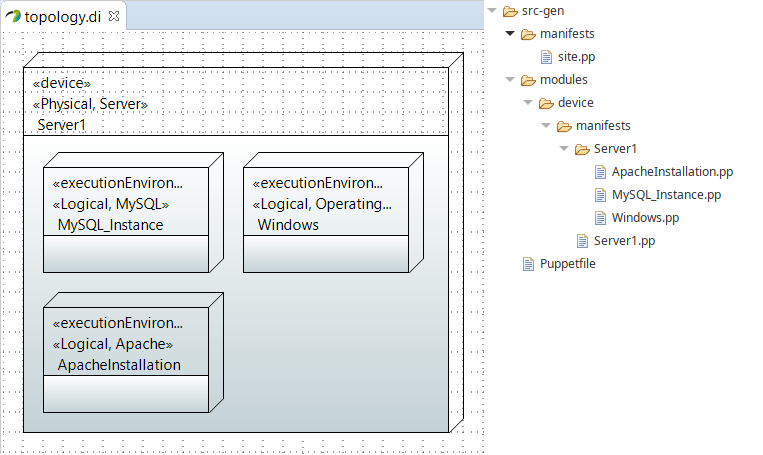
\includegraphics[width=0.8\textwidth]{figures/transformation_implementation/configuration_example0.png}
    \caption{Ejemplo de generación de archivos de Configuración.}
    \label{fig:transformation:configuration}
\end{figure}

En este ejemplo se puede ver la generación del archivo de configuración \textbf{Server1.pp}, que contiene la declaración del componente, e incluye al resto de los elementos que se encontrarán dentro del directorio \textbf{Server1}, un archivo de configuración por cada nodo Lógico. 
En la Figura \ref{fig:transformation:configuration_generated} se puede analizar el contenido de dichos archivos generados.

\begin{figure}[htbp]
    \centering
    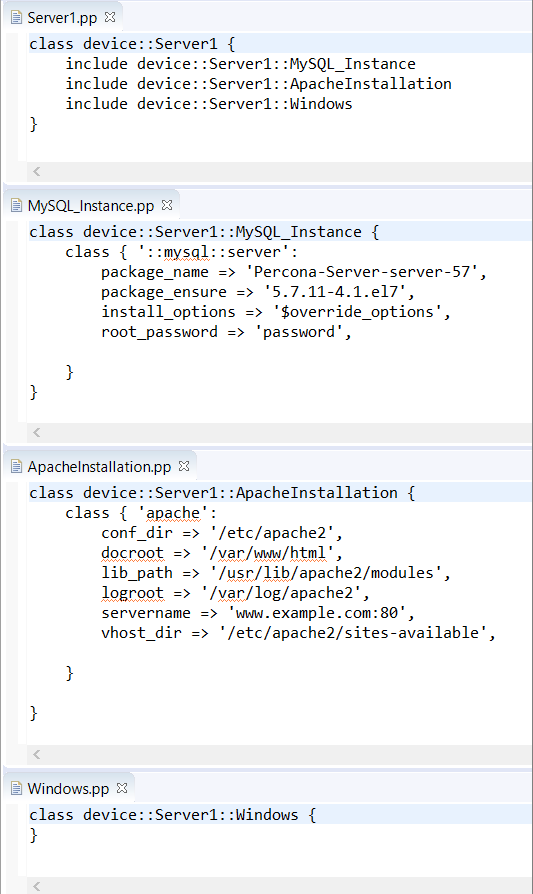
\includegraphics[width=0.75\textwidth]{figures/transformation_implementation/configuration_generation.png}
    \caption{Resultado de la transformación del modelo en la Figura \ref{fig:transformation:configuration}.}
    \label{fig:transformation:configuration_generated}
\end{figure}

Aquí se puede ver como el archivo de configuración del nodo Físico \textit{Server1.pp} es el encargado de incluir el resto de los componentes Lógicos \textit{MySQL\_Instance.pp}, \textit{ApacheInstallation.pp}, y \textit{Windows.pp}.
Tanto el componente de \textit{MySQL} como el de Apache genera su correspondiente archivo de configuración que será utilizado por el CMT, en el caso de \textit{Windows} se encuentra vacío debido a que no le fueron asignadas configuraciones de tipo \textit{File} o \textit{Registry}, que puedan ser aplicadas.

Como se mencionaba previamente, algunos elementos podrán generar tanto un archivo de configuración, como uno de información en texto plano, en este caso los componentes de servidor (Server1) y sistema operativo (Windows) también pueden generar estos archivos, en su correspondiente directorio (Figura \ref{fig:transformation:configuration_generated_1}).

\begin{figure}[htbp]
    \centering
    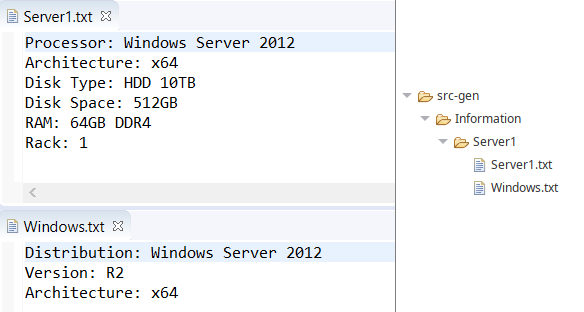
\includegraphics[width=0.75\textwidth]{figures/transformation_implementation/configuration_generation1.png}
    \caption{Archivos de información generados por los componentes servidor (Server1) y sistema operativo (Windows).}
    \label{fig:transformation:configuration_generated_1}
\end{figure}

La implementación de la transformación de los scripts se realizó de forma similar a los archivos de información, con el cuidado extra de mantener la sintaxis correcta de Puppet. Por ejemplo, el código de la transformación del archivo de configuración de Apache tiene la forma de la Figura \ref{fig:transformation:configuration_generator}.

\begin{figure}[htbp]
    \centering
    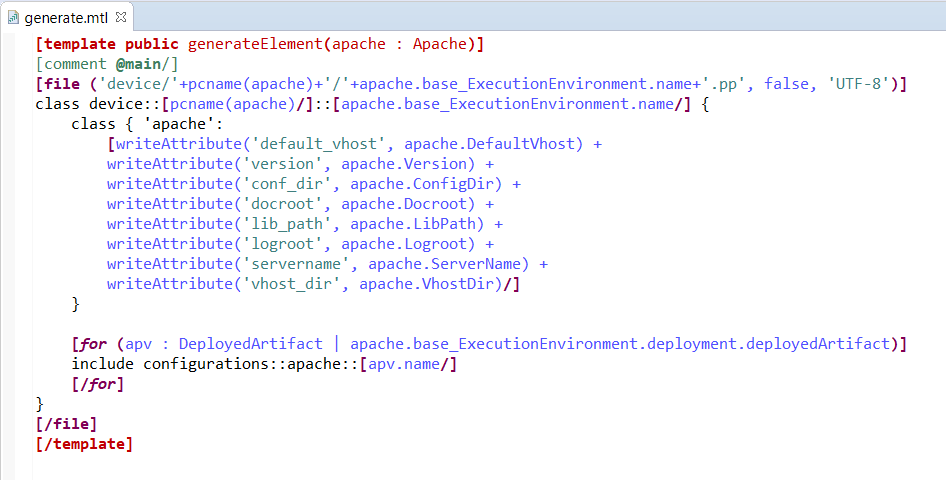
\includegraphics[width=\textwidth]{figures/transformation_implementation/configuration_generator.png}
    \caption{Código de la generación del archivo de configuración para el componente Lógico Apache.}
    \label{fig:transformation:configuration_generator}
\end{figure}

De igual forma que con los archivos de información, se utiliza un método auxiliar para dar formato a los atributos, además de realizar la inclusión de los artefactos de configuración asociados a ese elemento. 

Finalmente, se tiene la generación de los artefactos, o elementos de Configuración. En el ejemplo anterior se tenían nodos lógicos de MySQL, Apache, y Sistema Operativo, para ver esta última clase de elemento, se pueden agregar instancias de dichas configuraciones a cada uno de ellos. A modo de ejemplo, en la Figura \ref{fig:transformation:config_example} se agregó una instancia de base de datos MySQL, un host virtual de Apache, una configuración de archivo y una configuración de registro de Windows.

\begin{figure}[htbp]
    \centering
    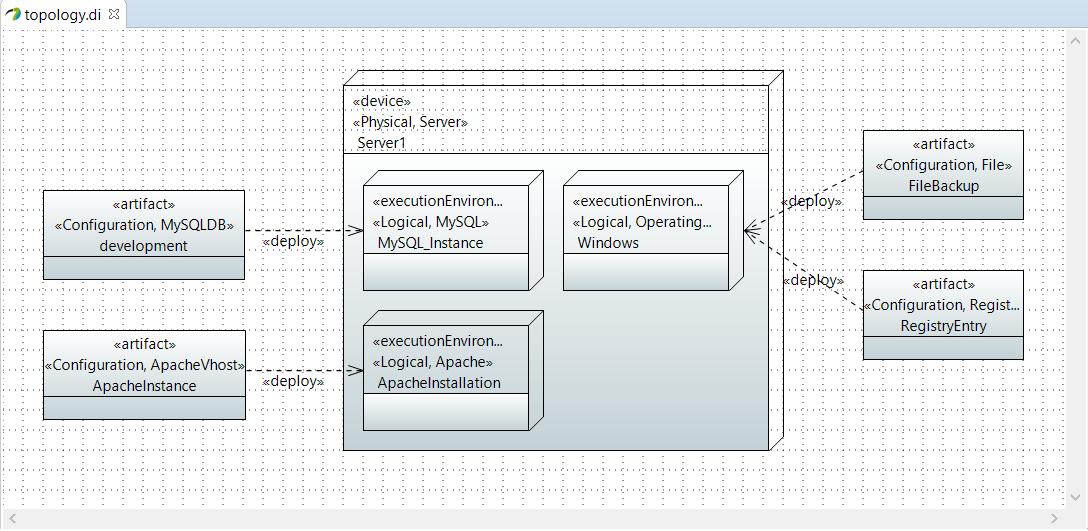
\includegraphics[width=\textwidth]{figures/transformation_implementation/full_config_example.png}
    \caption{Ejemplo de modelado con elementos de Configuración.}
    \label{fig:transformation:config_example}
\end{figure}

La transformación generada a partir de este modelo estará ubicada en el directorio \textbf{modules/configurations/manifests}, donde se creará un directorio por nodo lógico. Esta estructura se puede ver en la Figura \ref{fig:transformation:config_generation}.

\begin{figure}[htbp]
    \centering
    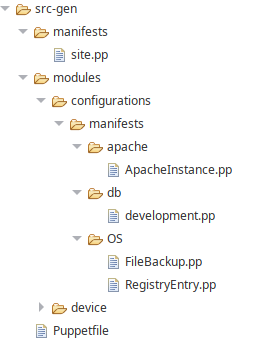
\includegraphics[width=0.4\textwidth]{figures/transformation_implementation/configuration_structure.png}
    \caption{Ejemplo de generación de archivos para los componentes de la Figura \ref{fig:transformation:config_example}.}
    \label{fig:transformation:config_generation}
\end{figure}

Como se puede apreciar en la Figura \ref{fig:transformation:configuration_generated_2}, el directorio OS contiene un archivo por cada artefacto que tiene desplegado sobre sí mismo. Si se analizan los resultados obtenidos en los archivos de configuración se puede ver que el contenido es similar al de los nodos lógicos, esto se debe a que siguen la misma sintaxis para definir dichos componentes en el CMT.

\begin{figure}[htbp]
    \centering
    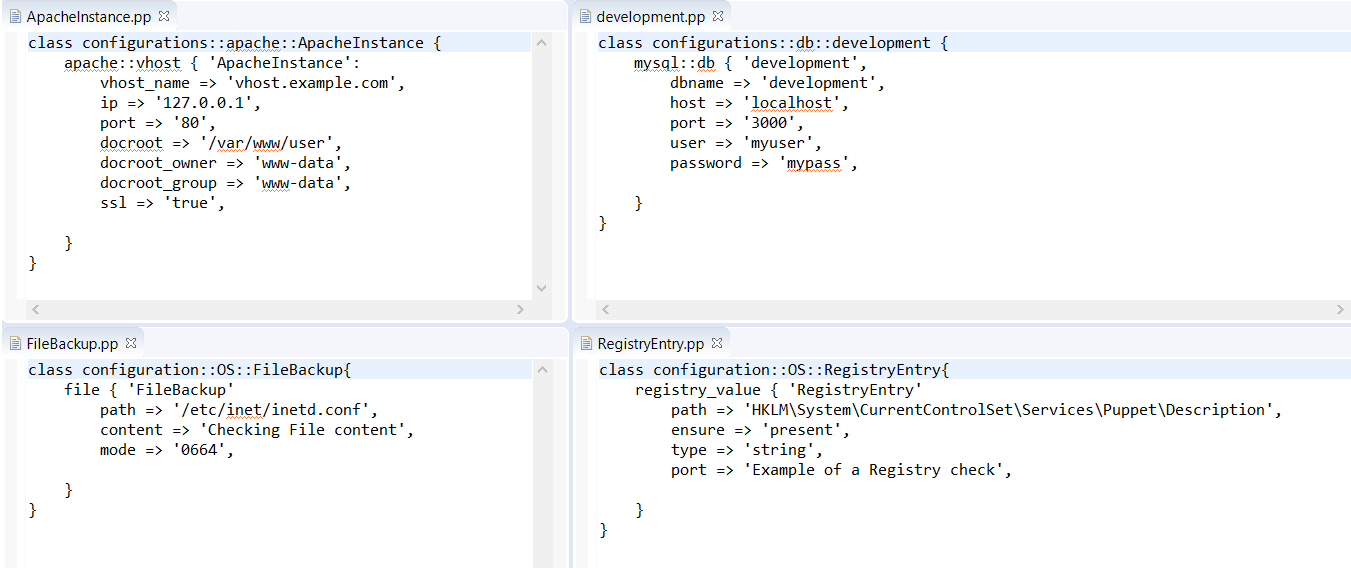
\includegraphics[width=\textwidth]{figures/transformation_implementation/configuration_generation2.png}
    \caption{Resultado de la transformación de los componentes de Configuración en la Figura \ref{fig:transformation:config_example}.}
    \label{fig:transformation:configuration_generated_2}
\end{figure}

Al mismo tiempo, si se analiza el código implementado para la transformación se puede ver que también es análogo al utilizado por el nodo lógico, por ejemplo, para el servidor virtual de Apache en la Figura \ref{fig:transformation:configuration_generator_2}.

\begin{figure}[H]
    \centering
    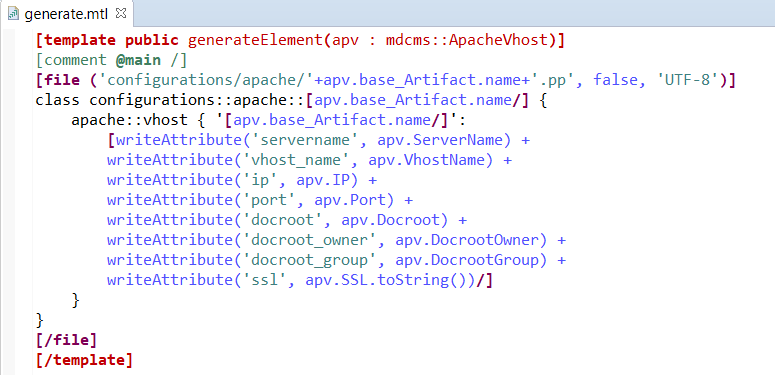
\includegraphics[width=\textwidth]{figures/transformation_implementation/configuration_generator2.png}
    \caption{Código de la generación del archivo de configuración para el componente de Configuración ApacheVhost.}
    \label{fig:transformation:configuration_generator_2}
\end{figure}

Con la generación de archivos de configuración obtenida, lo único que resta para aplicar la configuración mediante Puppet es utilizar estos archivos como entrada de la herramienta. Para esto existen varias opciones, por ejemplo mover los archivos generados al directorio adecuado, configurar la herramienta de configuración para que utilice el directorio de salida por defecto, o simplemente seleccionar como directorio destino de la transformación el directorio adecuado para Puppet. 

Para instalar dichas transformaciones en forma de plug-in es necesario generar un proyecto UI de Acceleo, lo cuál se puede realizar con la propia herramienta, seleccionando la opción Acceleo -> Create Acceleo UI Launcher Project, tal como se muestra en la Figura \ref{fig:transformation:acceleo_ui_project}. Por último, simplemente se exporta cada proyecto, tanto la transformación como el proyecto UI, de la misma forma que se describe en la sección anterior para el perfil UML.

\begin{figure}[htbp]
    \centering
    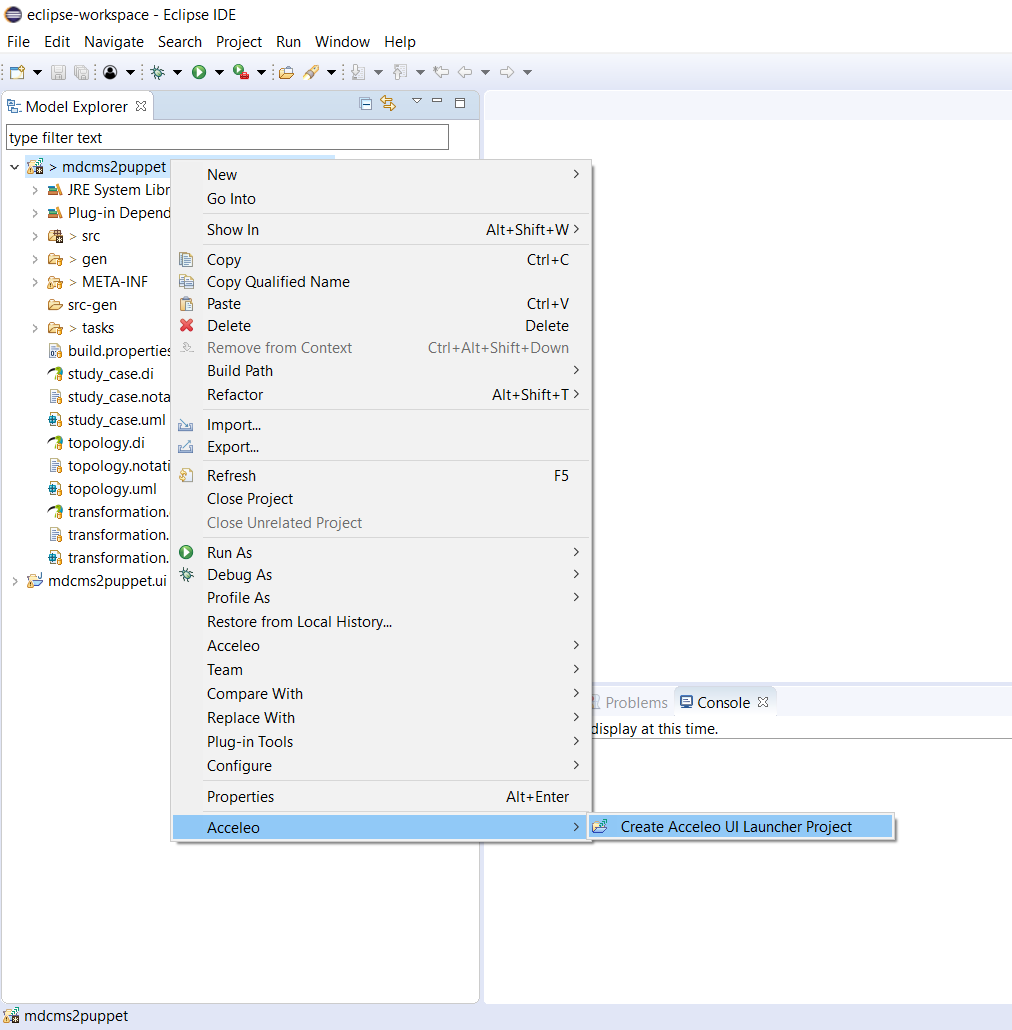
\includegraphics[width=\textwidth]{figures/transformation_implementation/acceleo_ui_project.png}
    \caption{Creación de proyecto UI de Acceleo.}
    \label{fig:transformation:acceleo_ui_project}
\end{figure}

\subsection{Resumen de transformaciones}

A continuación se presentan a modo de resumen dos tablas que mapean los distintos elementos del modelo con su resultado luego de ejecutar cada transformación.


En la tabla \ref{resumen:1} se pueden observar los elementos generados a partir de la transformación mdcms2puppet, mientras que en la tabla \ref{resumen:2} se encuentran los archivos de información generados por la transformación mdcms2info.
\begin{table}[H]
    \begin{adjustwidth}{-0.5in}{-1in}
        \centering
        \begin{center}
        \begin{tabular}{ll}
            Elemento de modelo & Elemento generado en transformación Puppet\\
            \hline
            PC & \texttt{modules/device/manifests/<pcname>.pp}\\
           Server & \texttt{modules/device/manifests/<servername>.pp}\\
            OperatingSystem & \texttt{modules/device/manifests/<devicename>/<osname>.pp}\\
           Apache & \texttt{modules/device/manifests/<devicename>/<apachename>.pp}\\
            Firewall & \texttt{modules/device/manifests/<devicename>/<firewallname>.pp}\\
            Java & \texttt{modules/device/manifests/<devicename>/<javaname>.pp}\\
            MySQL & \texttt{modules/device/manifests/<devicename>/<mysqlname>.pp}\\
            PostgreSQL & \texttt{modules/device/manifests/<devicename>/<postgresqlname>.pp}\\
            Tomcat & \texttt{modules/device/manifests/<devicename>/<tomcatname>.pp}\\
            ApacheVhost & \texttt{modules/configurations/manifests/apache/<vhostname>.pp}\\
            FirewallRule & \texttt{modules/configurations/manifests/firewall/<firewallname>.pp}\\
            JavaOracle & \texttt{modules/configurations/manifests/java/<javaoraclename>.pp}\\
            MySQLDB & \texttt{modules/configurations/manifests/db/<dbname>.pp}\\
            PSQLDB & \texttt{modules/configurations/manifests/db/<psqldbname>.pp}\\
            Tomcat & \texttt{modules/configurations/manifests/tomcat/<tomcatname>.pp}\\
            RegistryEntry & \texttt{modules/configurations/manifests/OS/<registryentryname>.pp}\\
            File & \texttt{modules/configurations/manifests/OS/<filename>.pp}  \\
        \end{tabular}
        \caption{Elementos generados en transformación Puppet}\label{resumen:1}
        \end{center}
    \end{adjustwidth}
\end{table}

\begin{table}
\begin{center}
\begin{tabular}{ll}
Elemento de modelo & Elemento generado en transformación Información\\
\hline
PC & \texttt{Information/<pcname>/<pcname>.pp}\\
Server & \texttt{Information/<servername>/<servername>.pp}\\
OperatingSystem & \texttt{Information/<devicename>/<operatingsystemname>.pp}\\
FreeForm & \texttt{Configuration/<freeformname>.pp}\\
Switch & \texttt{Information/<switchname>/<switchname>.pp}\\
Router & \texttt{Information/<routername>/<routername>.pp}\\
Peripheral & \texttt{Information/<peripheralname>/<peripheralname>.pp}\\
Firmware & \texttt{Information/<firmwarename>/<firmwarename>.pp}\\
\end{tabular}
\caption{Elementos generados en transformación Información}\label{resumen:2}
\end{center}
\end{table}